Dosud jsme vyšetřovali pouze ustálené stavy v elektrických obvodech, při kterých se větvové veličiny (proudy a napětí) mení periodicky.

Při změnách topologické nebo fyzikální struktury obvodu, mezi které například patří
\begin{itemize*}
\item spínací a vypínací děje (připojení nebo odpojení zdroje nebo spotřebiče)
\item poruchy (zkrat nebo rozpojení větve)
\end{itemize*}
se napětí a proudy mění neperiodicky. Tento stav obvodu nazýváme přechodným dějem. Obvod přechází z původního ustáleného stavu do nového ustáleného stavu. Tento proces je ilustrován na obrázku \ref{fig:prechodny_dej}
\begin{figure}[h!]
\centering
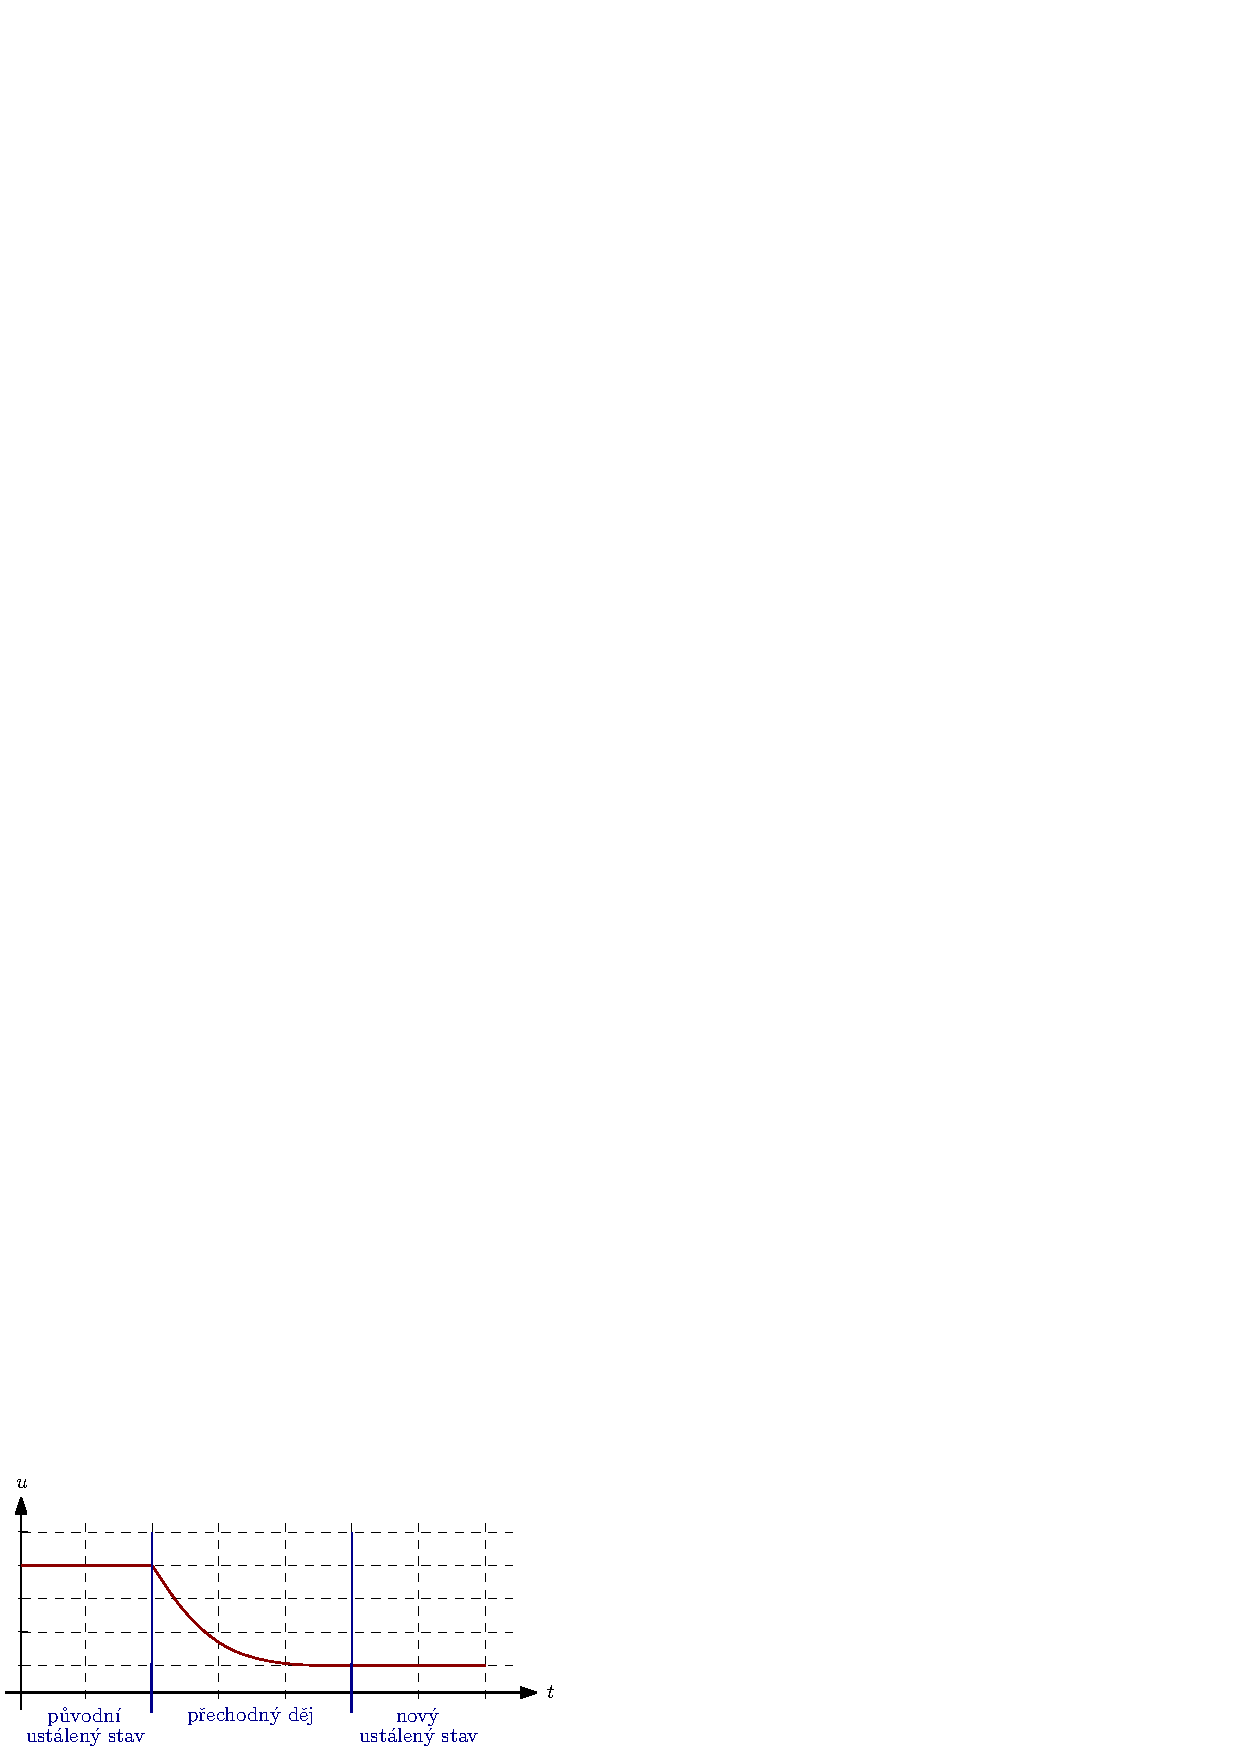
\includegraphics[]{prechodne_jevy/prechodny_dej.pdf}
\caption{Přechodný děj}
\label{fig:prechodny_dej}
\end{figure}

Rovnice pro analýzu přechodných dějů formulujeme zpravidla pro okamžité hodnoty napětí $u(t)$ a proudů $i(t)$. Jsou to obecně obyčejné integrodiferenciální rovnice a jejich řád je dán počtem prvků $L$ a $C$ v obvodu. Přechodný děj vzniká pouze v obvodech, které obsahují tzv. akumulační prvky, které jsou schopny akumulovat energii elektrického pole (kapacitory) nebo energii magnetického pole (induktory). V~obvodech obsahujících kromě zdroje pouze rezistory přechodný děj nevzniká, přeměna elektrické energie v tepelnou (Jouleovy ztráty) nastává okamžitě

Rozlišujeme přechodné děje v obvodech 1. řádu, které obsahují pouze jeden akumulační prvek (časový průběh napětí resp. proudu má pak exponenciální charakter) a v~obvodech vyšších řádů. V~obvodech 2. řádu může mít odezva obvodu exponenciální nebo kmitavý charakter.